\section{System Behavior}

This section describes how the system behaves as a whole and its overall functionality. 
It should give readers a clear understanding of the system's expected actions and reactions in different scenarios.

\subsection{General Overview}

The project is a navigation simulation where a user can place a starting position and ending position on a premade map based on a real life location (streets of city of Northridge) and watch the player's object car navigate from the starting position to the end with pathfinding. The player's car will have to navigate with other cars on the map that are going to their own locations to simulate traffic. We are able to pull a live-time image of current traffic and the streets through the TomTom API, which we used to build the premade map and have in the program. The cars were modelled and there are 5 different types of cars that can spawn. 

\subsection{Key Features and Functionality}
The program starts with a main menu, a Canvas with the title text and a button for the Northridge map scene. We can expand this menu with adding more map scenes for different areas and streets, but initially we wanted to use the TomTom API to pull a live image representing traffic that would be loaded onto the map. The user would input any location they want, and we would have a python code run through the image returned by the TomTom API for that location and make the 3d road scene for that location. Unfortunately, the issue we ran into here was that there is no distinction between highways and streets on the image, and there was no information on any traffic parts like street lights, stop signs, etc. Instead, we decided to have these presets and build the 3d map ourselves. 

\begin{figure}[htb]
    \centering
    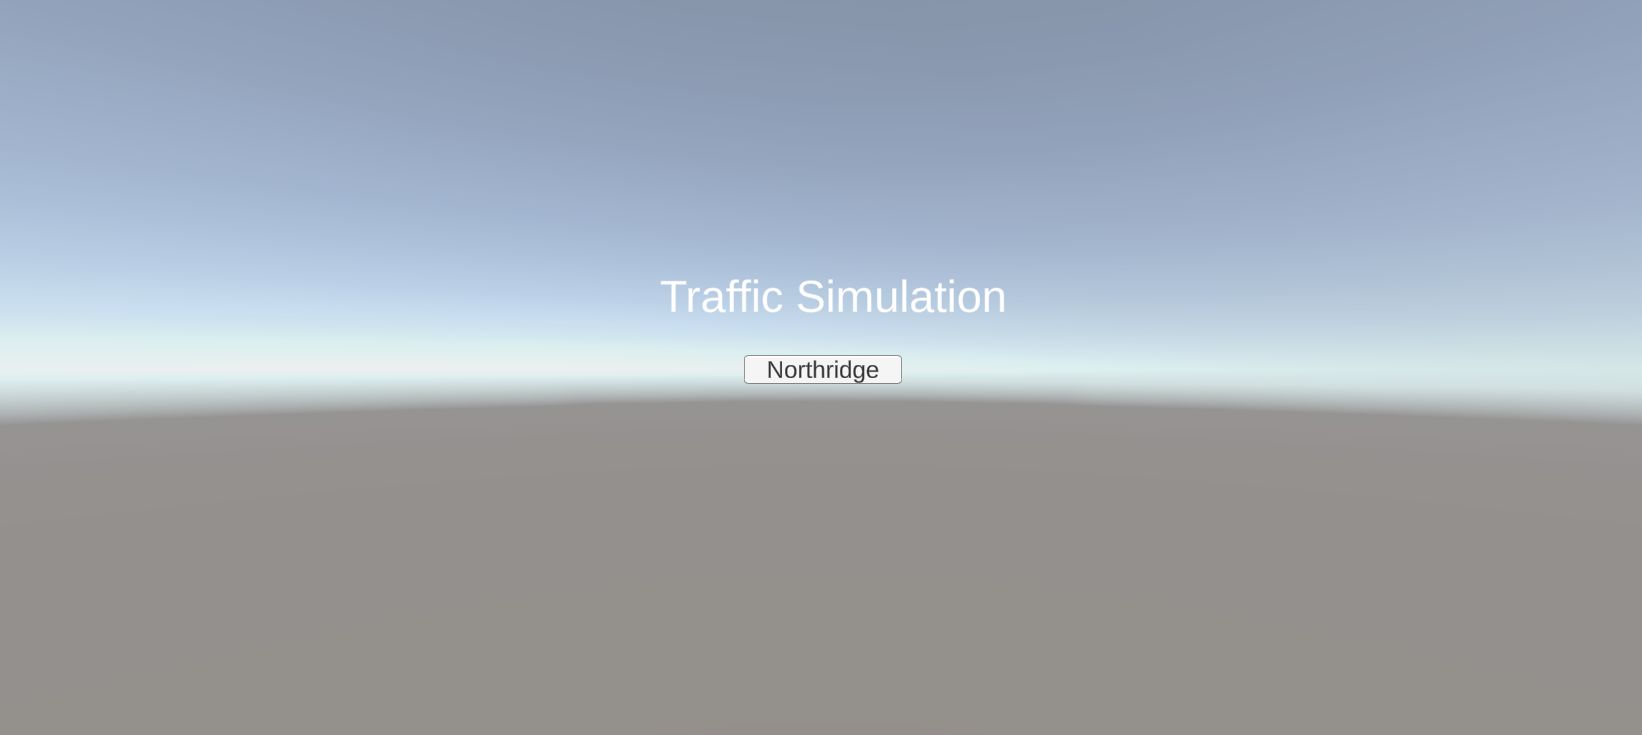
\includegraphics[width=10cm]{Images/MainMenu.png}
       \caption{The main menu.}
           \label{Fig:Main Menu}
\end{figure}

\begin{flushleft}
Once the user clicks on the Northridge button, the program switches to the Northridge scene that we made. Here, the user can choose a starting point for the car and an ending point for the car. This is achieved by the buttons "Start Marker" and "End Marker" on the side. Clicking on the Start Marker button then at a road on the map will place a green orb that represents the starting position. Click on the End Marker button then at a road on the map wll place a red orb that represents the ending position. 
\end{flushleft}

\begin{figure}[htb]
    \centering
    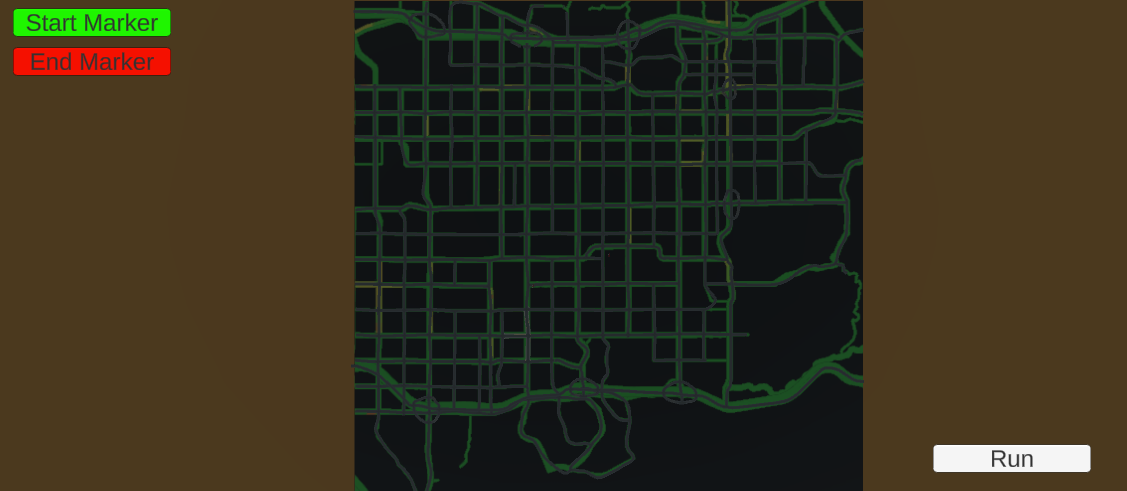
\includegraphics[width=10cm]{Images/Northridge1.png}
       \caption{The initial map and buttons "Start marker", "End Marker", and "Run".}
           \label{Fig:Game}
\end{figure}

\begin{flushleft}
When the user places both markers, then they can click the "Run" button to spawn their car on the road and start the simulation. Once the program starts running, the pathfinding class inside the car kicks in once it turns active at the event the users clicks run and the pathfinding will lock towards the positon of the End Position that the user made. The car will navigate towards the end position which it considers its goal, then stop there. Along the way, there can be car obstacles. All of the cars have a Nav Mesh Agent attached to them, and the cars that aren't the one the users chooses a start and end position for move towards randomized locations. When they reach that location, the goal position randomizes again and they move towards that one next. The spawned cars move on forever until the user stops the game.The cars are able to move along the roads because of the AI and Pathfinding Unity package that allows the roads to be "baked", which lets the car objects know which surfaces they can use pathfinding on and which they can't. Surfaces that can be traversed on need to be marked as static, hence all the road objects are static objects.
 \end{flushleft}

\begin{figure}[htb]
    \centering
    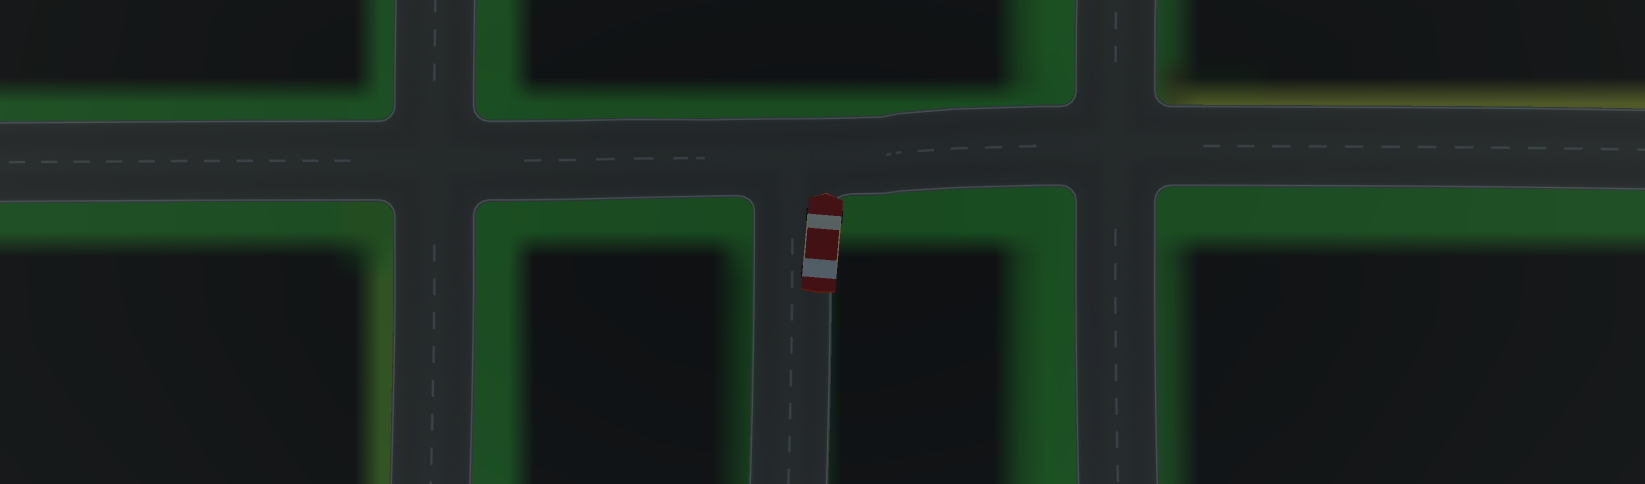
\includegraphics[width=10cm]{Images/Northridge2.png}
       \caption{The camera zooms in and follows the main car as it navigates to the end position.}
           \label{Fig:Game}
\end{figure}

\begin{figure}[htb]
    \centering
    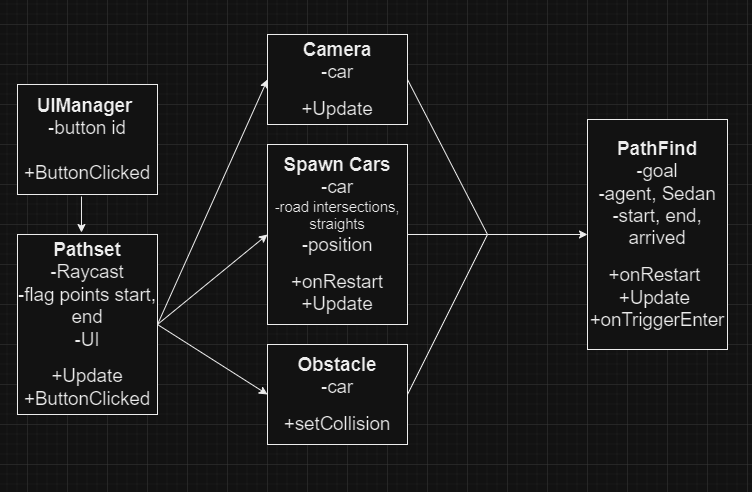
\includegraphics[width=10cm]{Images/UMLClasses.png}
       \caption{A UML Diagram for thec classes working inside the program.}
           \label{Fig:UML}
\end{figure}

\begin{flushleft}
The program uses the AI and Pathfinding packages in Unity, which need to be seperately downloaded. The UI Manager class handles the scene switch from the main menu with the maps, then how the user can choose a starting position and ending position as discussed earlier. Here, the program takes in the button id of the button clicked, which are ids for the starting point, ending point, and run button. The run button will not start unless both the start and end destinations have been set by the user, there are no default positions that can be run if the user doesn't put in anything. The UI has the class PathSet within it as well, where it will take in the position of where the user set the start position and the end position considered "flag points start, end" from a raycast sent from the user's click onto a road. The road's position is sent back from the raycast, then the flag point is set there. Whichever flag point it is is determined by the button id from the UIManager.
 \end{flushleft}

\begin{flushleft}
Once the positions have been set and the user chooses to run the program, three classes run simultaneously to set the scene. Firstly, the camera object is set to follow the car object with an offset, where update will move the camera onto the car with the offset to make it follow it the whole way. Secondly, the spawn cars class instantiates prefabs of cars onto the map. How the code handles this is setting an array of the different type of car prefabs that a random range of 0-4 chooses from, then that car is instantiated onto a random position of a road intersection. Initially, we wanted cars to have the option to spawn onto either a straight road or on an intersection (hence the road intersections, straights) however the straight roads that are built into the map have a local position of (0,0,0). Taking in the object's position would just return (0,0,0), then all cars would spawn from that point of the map globally regardless of if randomizing which road straight they spawn from has been successfully initialized. This is why instead we are spawning cars from just road intersections, as road intersections have global transform positions attached to them instead of the local positions the road straights have. There was a lot of learning about parent and child relationships with this project. The onRestart represents the event that the pathFind will wait for the cue for. The obstacle class set the nav mesh agents on all the spawned cars that they can recognize eachother as collisions or obstacles that no car can phase through one another. After those classes have run, then the onRestart event is called the the PathFind finally runs.
 \end{flushleft}

\begin{flushleft}
The Pathfind takes in the end position or goal that has been set by the user, and initializes a nav mesh agent to the Sedan that the main player navigates. It also takes in the start position where the Sedan will start from, the end position where the Sedan will go towards, and the arrived that is the end position that the Sedan will stop when it gets to its destination. At Update, the agent's destination moves towards the end position working with pathfinding. The onTriggerEnter should make the Sedan recognize that it has reached it's destination and let a "You've arrived" text pop up, but the position most likely isn't set correctly for the Sedan to recognize it's arrived which is a continuing issue that can be fixed, just ran out of time. The user's Sedan is conscious of other cars and avoids collisions because every car is set with a nav mesh agent (to which, human error is also another component of traffic that should be consideredin a simulation) and moves around them or drives behind them slowly at a distance.
 \end{flushleft}


\begin{flushleft}
Improvements we can make to the system could be some way to organize the positions better that they can be easier taken, have an option for the user to choose positions outside of the road objects and return the nearest road object to the marker, and make the navigation a little more restrictive that cars don't drive in the middle of the road.
 \end{flushleft}